\documentclass{article}
\usepackage{amsthm,amsmath,amsfonts,lipsum}
\usepackage[T1]{fontenc}
\usepackage{beramono}
\usepackage{listings}
\usepackage{fontawesome5}
\usepackage{adjustbox}
\usepackage{mathabx}
\usepackage{thmtools}
\usepackage{import}
\usepackage{graphicx}
\usepackage{setspace}
\usepackage{geometry}
\usepackage{physics}
\usepackage{float}
\usepackage[english]{babel}
\usepackage{framed}
\usepackage[dvipsnames,x11names]{xcolor}
\usepackage{tcolorbox}
\usepackage{fancyhdr}
\usepackage{hyperref}
\usepackage{booktabs}
\usepackage{enumitem}
\usepackage{cancel}
\usepackage{background}
\usepackage{units}
\usepackage{textcomp}

% Configuring the background
\backgroundsetup{
  scale=1, % Optional, scale if needed
  color=black, % Optional, set the image color, can be omitted
  opacity=0.18, % Optional, adjust opacity for watermark effect
  angle=0,
  position=current page.center, % Center the image on the page
  contents={
\includegraphics[width=1.75\paperwidth, height=1.75\paperheight, keepaspectratio]{ninym_ralei_leaf (watermarked by AlexanderTheMango)}} % Keeps aspect ratio and scales to fill the page
}

% Colours
\definecolor{darkgreen}{rgb}{0.0, 0.5, 0.0}
\definecolor{Firebrick}{rgb}{0.698, 0.132, 0.203}
\definecolor{Crimson}{rgb}{0.862745, 0.078431, 0.235294} % Crimson color
\definecolor{lightred}{rgb}{1.0, 0.819608, 0.819608} % Light red for background
\definecolor{MediumPurple}{rgb}{0.576, 0.439, 0.859}
\definecolor{chocolate}{rgb}{0.82, 0.41, 0.12} % Chocolate color definition
\definecolor{myframecolor}{rgb}{0.25, 0.41, 0.88} % RoyalBlue
\definecolor{mybackgroundcolor}{rgb}{0.68, 0.85, 0.90} % LightSkyBlue
% Define the Navy color
\definecolor{Navy}{rgb}{0.0, 0.0, 0.5}

% Define custom tcolorbox styles for notes
\tcbuselibrary{skins, breakable}
\newtcolorbox{definitionbox}{colframe=RoyalBlue, colback=blue!5!white, title=Definition}
\newtcolorbox{examplebox}{colframe=ForestGreen, colback=green!5!white, title=Example}
\newtcolorbox{notebox}{colframe=RedOrange, colback=orange!5!white, title=Note}
\newtcolorbox{theorembox}{colframe=RoyalPurple, colback=purple!5!white, title=Theorem}

\newtcolorbox{propositionbox}{colframe=myframecolor, colback=mybackgroundcolor!20!white, title=Proposition}
\newtcolorbox{remarkbox}{colframe=MidnightBlue, colback=blue!10!white, title=Remark}
\newtcolorbox{corollarybox}{colframe=OliveGreen, colback=green!10!white, title=Corollary}
\newtcolorbox{warningbox}{colframe=Crimson, colback=lightred, title=Warning}
\newtcolorbox{proofbox}{colframe=Black, colback=gray!10!white, title=Proof}
\newtcolorbox{questionbox}{colframe=Teal, colback=teal!10!white, title=Question}
\newtcolorbox{tipbox}{colframe=Goldenrod, colback=yellow!10!white, title=Tip}
\newtcolorbox{exercisebox}{colframe=darkgreen, colback=green!5!white, title=Exercise}
\newtcolorbox{solutionbox}{colframe=DodgerBlue4, colback=blue!5!white, title=Solution}
\newtcolorbox{algorithmbox}{colframe=Navy, colback=blue!10!white, title=Algorithm}
\newtcolorbox{conceptbox}{colframe=chocolate, colback=brown!10!white, title=Concept}
\newtcolorbox{illustrationbox}{colframe=Firebrick, colback=red!10!white, title=Illustration}
\newtcolorbox{intuitionbox}{colframe=MediumPurple, colback=purple!10!white, title=Intuition}
\newtcolorbox{answerbox}{colframe=RoyalBlue, colback=blue!10!white, title=Answer}

% Geometry settings
\geometry{letterpaper, portrait, includeheadfoot=true, hmargin=1in, vmargin=1in}
\onehalfspacing

% Header and footer
\pagestyle{fancy}
\fancyhf{}
\lhead{MAT232 - Lecture Notes}
\rhead{\thepage}
\lfoot{University of Toronto Mississauga}
\rfoot{\today}

% Document starts
\begin{document}
\renewcommand{\familydefault}{\rmdefault}

\begin{titlepage}
    \null % This is a TeX command that does nothing but is necessary for vfill to work correctly
    \vfill
    \begin{center}
        {\fontsize{40}{48}\selectfont \bfseries MAT232 - Lecture 13}
        \vspace{20pt} \\
        {\LARGE after partial derivatives?} \\
        \vspace{20pt}
        \textbf{AlexanderTheMango}
        \vspace{8pt}
        \\ Prepared for February 24, 2025
    \end{center}
    \vfill
\end{titlepage}


\newpage
\setcounter{page}{0}
\tableofcontents
\newpage

\begin{titlepage}
    \null % Ensures proper alignment with vfill
    \vfill
    \begin{center}
        {\Huge \textbf{Definitions and Theorems}} \\[20pt]
        \rule{\textwidth}{0.5mm} \\[15pt]
        {\Large \textit{Straight from the textbook — lots of fluff this time, more than what we need!}} \\[15pt]
        \rule{\textwidth}{0.5mm} \\[15pt]
        \textbf{Quick recap before diving into the lecture.}
    \end{center}
    \vfill
\end{titlepage}


\section*{Polar Coordinates - Key Theorems}
\addcontentsline{toc}{section}{Polar Coordinates - Key Theorems}

\subsection*{Converting Points between Coordinate Systems}
\addcontentsline{toc}{subsection}{Converting Points between Coordinate Systems}
\begin{theorembox}
    Given a point \( P \) in the plane with Cartesian coordinates \( (x,y) \) and polar coordinates \( (r,\theta) \), the following conversion formulas hold true:
    \[
    x = r \cos\theta \quad \text{and} \quad y = r \sin\theta,
    \]
    \[
    r^2 = x^2 + y^2 \quad \text{and} \quad \tan\theta = \frac{y}{x}.
    \]
    These formulas can be used to convert between rectangular and polar coordinates.
\end{theorembox}

\subsection*{Uniqueness of Polar Coordinates}
\addcontentsline{toc}{subsection}{Uniqueness of Polar Coordinates}
\begin{propositionbox}
    Every point in the plane has an infinite number of representations in polar coordinates. Specifically, the polar coordinates \( (r, \theta) \) of a point are not unique.
    
    \begin{remarkbox}
        For example, the polar coordinates \( (2, \pi/3) \) and \( (2, 7\pi/3) \) both represent the same point in the rectangular coordinate system. Additionally, the value of \( r \) can be negative. Therefore, the point with polar coordinates \( (-2, 4\pi/3) \) represents the same rectangular point as \( (2, \pi/3) \).
    \end{remarkbox}
\end{propositionbox}

\subsection*{Symmetry of Polar Curves}
\addcontentsline{toc}{subsection}{Symmetry of Polar Curves}
\begin{theorembox}
    Polar curves can exhibit symmetry similar to those in rectangular coordinates. The key symmetries to identify are:
    \begin{itemize}
        \item \textbf{Symmetry with respect to the polar axis:} A curve is symmetric with respect to the polar axis if replacing \( \theta \) with \( -\theta \) in its equation yields the same curve.
        \item \textbf{Symmetry with respect to the line \( \theta = \frac{\pi}{2} \):} A curve is symmetric with respect to the line \( \theta = \frac{\pi}{2} \) if replacing \( \theta \) with \( \pi - \theta \) yields the same curve.
        \item \textbf{Symmetry with respect to the pole (origin):} A curve is symmetric with respect to the pole if replacing \( r \) with \( -r \) yields the same curve.
    \end{itemize}
\end{theorembox}

\begin{titlepage}
    \null % Ensures proper alignment with vfill
    \vfill
    \begin{center}
        {\Huge \textbf{Let’s Get Started}} \\[20pt]
        \rule{\textwidth}{0.5mm} \\[15pt]
        {\Large \textit{Time to dive into the lecture notes.}} \\[15pt]
        \rule{\textwidth}{0.5mm} \\[15pt]
        \textbf{Grab your pen or pencil, and let’s break this down step by step.}
    \end{center}
    \vfill
\end{titlepage}

\setcounter{page}{2}
\normalsize

\section*{Plotting Polar Coordinates}

\subsection*{Recall the Content from Last Lecture}
\addcontentsline{toc}{subsection}{Recall the Content from Last Lecture}
\begin{notebox}
Converting between Cartesian coordinates \( (x, y) \) and Polar coordinates \( (r, \theta) \):

\begin{algorithmbox}
    \textbf{From Cartesian to Polar:}
    \[
        r = \sqrt{x^2 + y^2}, \quad \theta = \arctan\left(\frac{y}{x}\right)
    \]
    
    \textbf{From Polar to Cartesian:}
    \[
        x = r\cos\theta, \quad y = r\sin\theta
    \]
\end{algorithmbox}

\textbf{Converting Between Degrees and Radians:}
\begin{algorithmbox}
    \begin{itemize}
        \item \textbf{Degrees to Radians:} Multiply by \( \dfrac{\pi}{180^{\circ}} \)
        \[
        \text{Radians} = \text{Degrees} \times \dfrac{\pi}{180^\circ}
        \]
        \item \textbf{Radians to Degrees:} Multiply by \( \dfrac{180^\circ}{\pi} \)
        \[
        \text{Degrees} = \text{Radians} \times \dfrac{180^\circ}{\pi}
        \]
    \end{itemize}
\end{algorithmbox}
\end{notebox}

\subsection*{Understanding the Convention for \( r \) in Polar Coordinates}
\addcontentsline{toc}{subsection}{Understanding the Convention for \( r \) in Polar Coordinates}

\begin{conceptbox}
In polar coordinates, a point is represented as \( (r, \theta) \), where:
\begin{itemize}
    \item \( r \) is the radial distance from the origin (how far the point is from the origin).
    \item \( \theta \) is the angle, measured counterclockwise from the positive x-axis.
\end{itemize}

\begin{notebox}
    \subsubsection*{Special Case: When \( r \) is Negative}
    \begin{itemize}
        \item A negative \( r \) in \( (-r, \theta) \) is interpreted as the point being reflected through the origin.
        \item The equivalent representation is:
        \[
        (-r, \theta) = (r, \theta + 180^\circ)
        \]
        or in radians:
        \[
        (-r, \theta) = (r, \theta + \pi)
        \]
    \end{itemize}
\end{notebox}

\begin{intuitionbox}
    \begin{itemize}
        \item Reflecting \( (r, \theta) \) through the origin is the same as rotating the point by \( 180^\circ \) (or \( \pi \) radians).
        \item This property simplifies polar plots by offering alternate representations of the same point.
    \end{itemize}
\end{intuitionbox}
\end{conceptbox}

\subsection*{Example: Plotting Points}
\addcontentsline{toc}{subsection}{Example: Plotting Points}

\begin{examplebox}
Let us plot the following points in polar coordinates:
\[
(3, -45^\circ), \quad (3, 225^\circ), \quad (4, 330^\circ), \quad (1, -45^\circ)
\]

\begin{algorithmbox}
    \textbf{Step-by-Step Process:}
    \begin{enumerate}
        \item For each point, identify \( r \) and \( \theta \).
        \item If \( \theta \) is negative or exceeds \( 360^\circ \), convert it to a standard range:
        \[
        \theta \in [0^\circ, 360^\circ)
        \]
        using \( \theta = \theta + 360^\circ \) (for negative angles) or subtracting \( 360^\circ \) (for angles over \( 360^\circ \)).
        \item Plot the point by measuring \( \theta \) counterclockwise from the positive x-axis and placing it at a distance \( r \) from the origin.
    \end{enumerate}
\end{algorithmbox}

\begin{solutionbox}
    \begin{itemize}
        \item For \( (3, -45^\circ) \): Add \( 360^\circ \) to \(-45^\circ\) to convert \( \theta \) to \( 315^\circ \). Plot as \( (3, 315^\circ) \).
        \item For \( (3, 225^\circ) \): Already within the standard range, so plot directly.
        \item For \( (4, 330^\circ) \): Angle is standard, so plot directly.
        \item For \( (1, -45^\circ) \): Add \( 360^\circ \) to \(-45^\circ\), yielding \( (1, 315^\circ) \).
    \end{itemize}
    
    \begin{figure}[H]
        \centering
        \begin{minipage}{0.3\textwidth}
            \centering
            
\includegraphics[width=\textwidth]{plot points.png}
            \caption{Colour Legend}
            \label{fig:image1}
        \end{minipage}%
        \hspace{0.04\textwidth} % Adds horizontal space between the images
        \begin{minipage}{0.65\textwidth}
            \centering
            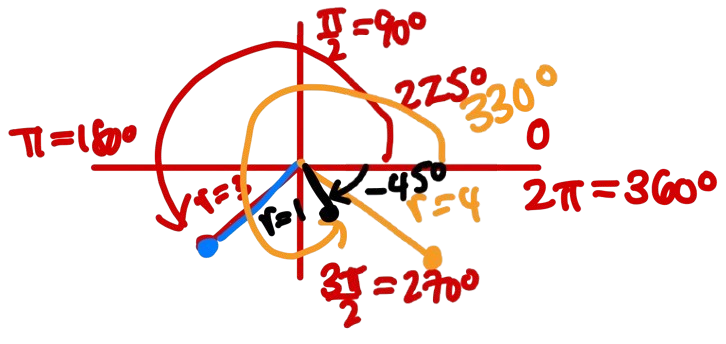
\includegraphics[width=\textwidth]{plot points example.png}
            \caption{Polar Coordinates Plot and ``Trajectories''}
            \label{fig:image2}
        \end{minipage}
    \end{figure}    
\end{solutionbox}
\end{examplebox}

\begin{tipbox}
    Ensure to label points clearly on the polar grid, and verify angle conversions and reflections for accuracy.
\end{tipbox}

\subsection*{Example: Converting from Polar Coords to Cartesian Coords}
\addcontentsline{toc}{subsection}{Example: Converting from Polar Coords to Cartesian Coords}

\begin{examplebox}
Find the \textbf{rectangular coordinates} (or Cartesian coordinates) of the point \( p \) whose polar coordinates are \( (6, \frac{\pi}{3}) \).

\begin{solutionbox}
To convert from polar to Cartesian coordinates, we use the following formulas:

\[
    x = r \cos \theta
\]
\[
    y = r \sin \theta
\]

Substitute the given values for \( r = 6 \) and \( \theta = \dfrac{\pi}{3} \):

\begin{itemize}
    \item For \( x \):
    \[
        x = 6 \cos \left( \frac{\pi}{3} \right) = 6 \left( \frac{1}{2} \right) = 3
    \]
    \item For \( y \):
    \[
        y = 6 \sin \left( \frac{\pi}{3} \right) = 6 \left( \frac{\sqrt{3}}{2} \right) = 3\sqrt{3}
    \]
\end{itemize}

Thus, \( (x, y) = (3, 3\sqrt{3}) \).

\begin{answerbox}
    The cartesian coordinates of the point are \( (x, y) = (3, 3\sqrt{3}) \).
\end{answerbox}

\end{solutionbox}
\end{examplebox}

\section*{Converting from Cartesian Coordinates to Polar Coordinates}
\begin{examplebox}
Find the polar coordinate of the point \( p \) whose rectangular coordinates are \( -2, 2\sqrt{3} \).

\begin{solutionbox}
Recall that (the circle equation):
\[
    x^2 + y^2 = r^2
\]
It follows that:
\[
    (-2)^2 + (2\sqrt{3})^2 = r^2
\]
\[
    4 + 4 \cdot 3 = r^2
\]
\[
    16 = r^2
\]
\[
    \pm \sqrt{16} = r 
\]
\[
    r = \pm 4
\]
Note that the radius is positive. Thus:
\[
    r = 4 \text{.}
\]
Recall that:
\[
    \tan(\theta) = \frac{y}{x}
\]
\[
    \tan(\theta) = \frac{2\sqrt{3}}{-2}
\]
\[
    \tan(\theta) = -\sqrt{3}
\]
\begin{notebox}
Note that:
\[
    \arctan(\frac{y}{x}) = \theta, \quad \frac{\pi}{2} < \theta < \frac{\pi}{2}
\]
\end{notebox}
\begin{tipbox}
Manually determining \( \theta \) from \( \tan(\theta) = \sqrt{3} \).

Note the special angles (in radians):
\begin{itemize}
    \item \( 0 \) 
    \item \( \frac{\pi}{6} \) 
    \item \( \frac{\pi}{4} \)
    \item \( \frac{\pi}{3} \)
    \item \( \frac{\pi}{2} \)
\end{itemize}
Check:
At \( \theta = \frac{\pi}{6} \),
\[
    LHS = \dfrac{\sin(\frac{\pi}{6})}{\cos(\frac{\pi}{6})}
\]
\[
    LHS = \dfrac{\frac{1}{2}}{\frac{\sqrt{3}}{2}}
\]
\[
    LHS = (\dfrac{1}{2})(\dfrac{2}{\sqrt{3}})
\]
\[
    LHS = \frac{1}{\sqrt{3}}
\]
\[
    RHS = \sqrt{3}
\]
Clearly, \( LHS = \frac{1}{\sqrt{3}} \neq \sqrt{3} = RHS \).
So, \( \theta \neq \frac{\pi}{6} \).

Now, do the same to check that \( \theta \) is indeed \( \sqrt{3} \).
[do that here!]
\end{tipbox}

We now have \( (r, \theta) = (4, -\frac{\pi}{3 = -60\text{\textdegree}})\). \\
\\
We don't want to retain the negative! \\
\\
So, the fix\dots
\[
    (4, -\frac{\pi}{3} + \pi = -60\text{\textdegree} + 180\text{\textdegree}) = (4, \frac{2\pi}{3} = 120\text{\textdegree})
\]
\end{solutionbox}
\end{examplebox}

\begin{tipbox}
When practicing for this course, you are encouraged to leverage any available graphing websites and/or software. \\
\\
Ideally, you want to know how to draw lines and circles.
\end{tipbox}

\section*{Polar Curves}
\begin{examplebox}
Consider \( r = f(\theta) \). \\
\\
Sketch the following functions: \\
(a) \( r = 1 \) \\
(b) \( \theta = \frac{\pi}{4} \) \\
(c) \( r = \theta, \quad \theta \geq 0 \) \\
(d) \( r = \sin(\theta) \) \\
(e) \( r = \cos(2\theta) \) \\
\\
\end{examplebox}

(a)
\begin{solutionbox}
Here, \( r = 1 \) and \( \theta \) is an arbitrary angle. \\
\\
Converting from a polar-coordinate curve to a cartesian-coordinate equation:
\[
    x^2 + y^2 = r^2 = 1^2 = 1
\]
Clearly, we are working with the unit cirle.

\textbf{self-note: actually show the illustration as andie drew on the lecture notes}
\end{solutionbox}

(b)
\begin{solutionbox}
    [fill this in]
\end{solutionbox}

(c) \( r = \theta, \quad \theta \geq 0 \)
\begin{solutionbox}
As \( r \to \infty \), \( \theta \) increases.
\[
    r = f(\theta)
\]
\[
    \pi \doteq 3.14
\]
\[
\begin{array}{c|c|c|c|c|c}
\theta & 0 & \frac{\pi}{6} & \frac{\pi}{4} & \frac{\pi}{3} & \frac{\pi}{2} \\
\hline
r & 0 & \doteq 1 & \doteq 1.2 & \doteq 1.4 & \doteq 1.5 \\
\end{array}
\]

Check out the illustration:
[add-illustration-here] \\
\\
Now, converting from polar coordinates to cartesian coordinates:
\[
    x^2 + y^2 = r^2
\]
\[
    \sqrt{x^2 + y^2} = r
\]
[and also add the other equation]
\end{solutionbox}

(d) \( r = \sin\theta \)
\begin{solutionbox}
\[
\begin{array}{c|c|c|c|c|c}
\theta & 0 & \frac{\pi}{6} & \frac{\pi}{4} & \frac{\pi}{3} & \frac{\pi}{2} \\
\hline
r & 0 & \frac{1}{2} & \frac{1}{\sqrt{2}} & \frac{\sqrt{3}}{2} & 1 \\
\end{array}
\]
Just use the table to directly plot the points for the graph! \\
\\
\textbf{add-illustration-here}
We now need an equation that will help us get rid of \( r = \sin\theta \). Consider the possibilities:
\begin{itemize}
    \item \( x = r\cos\theta \)
    \item \( y = r\sin\theta \)
    \item \( \frac{y}{r} = \sin\theta \)
\end{itemize}

\[
    r = \sin\theta
\]
\[
    r = \frac{y}{r}
\]
\[
    r^2 = y
\]
\( x^2 + y^2 = r^2 \)
So,
\[
    x^2 + y^2 = y \text{.}
\]
\begin{propositionbox}
Recall how to complete the square from Grade 10 math:
\textbf{self-note: add that here to reference}
\end{propositionbox}
Proceed to complete the square:
\[
    x^2 + y^2 - y + \frac{1}{4} = \frac{1}{4}
\]
step no. 1: \( -\frac{1}{2} \) \\
step no. 2: \( (-\dfrac{1}{2})^2 = \frac{1}{4} \).
Recall that:
\[
    (y + a)^2 = (y + a)(y + a)
\]
\[
    = y^2 + 2ay + a^2
\]
This would represent the \( y^2 - y + \frac{1}{4} \) part.

Note that the \( (y - a)^2 \) represents the \( -\frac{1}{2} \) 

result:
\[
    x^2 + (y - \frac{1}{2})^2 = \frac{1}{4}
\]
Centre: \( (0, \frac{1}{2}) \) \\
Radius: \( r = \frac{1}{2} \) \\

\end{solutionbox}

\begin{exercisebox}
Try:
\[
    r = \cos\theta
\]
under the same context as denoted for the above questions.
\end{exercisebox}

\section*{The Derivative of a Polar Curve}
\subsection*{Tangents to Polar Curves}
\begin{definitionbox}
\begin{notebox}
Recall that polar curves are defined by:
\[
    r = f(\theta)
\]
\end{notebox}
\[
    x = r\cos\theta = f(\theta) \cos\theta
\]
\[
    y = r\sin\theta = f(\theta) \sin\theta
\]
\begin{intuitionbox}
The goal is to have everything on \( x \) depend on \textbf{one} parameter. \\
\\
Do the exact same thing on \( y \).
\end{intuitionbox}

So, 
\[
    \dfrac{dy}{dx} = \dfrac{\dfrac{dy}{d\theta}}{\frac{dx}{\dfrac{d}{\theta}}}.
\]
We want require \( \frac{dx}{d\theta} \neq 0 \).

So\dots
\[
    \frac{dy}{dx} = \frac{\frac{dy}{d\theta}}{\frac{dx}{d\theta}}
\]
\[
    = \dfrac{\frac{df(\theta)}{d\theta} \sin\theta + \cos\theta f(\theta)}{\frac{df(\theta)}{d\theta} \cos\theta - \sin\theta f(\theta)}
\]
So,
\[
    \frac{dy}{dx} = \frac{\frac{dy}{d\theta}}{\frac{dx}{d\theta}} = \dfrac{\frac{dr}{d\theta} \sin\theta + r \cos\theta}{\frac{dr}{d\theta} \cos\theta - r \sin\theta}
\]
(subbed \( r \) in for \( f(\theta) \)).
\underline
\\
{Conclusion:}
\begin{itemize}
    \item Horizontal Tangents: \( \frac{dy}{d\theta} = 0, \quad \frac{dx}{d\theta} \neq 0 \)
    \item Vertical Tangents: \( \frac{dx}{d\theta} = 0, \quad \frac{dy}{d\theta} \neq 0 \)
    \item Singular Points (discard; we will not be doing further analysis for this case in MAT232): \( \frac{dy}{d\theta} = \frac{dx}{d\theta} = 0 \)
\end{itemize}

\end{definitionbox}

\section*{Examples}
\begin{examplebox}
Find the \textbf{vertical tangent} angles of the polar curve \( r = 1 - \cos\theta, \quad 0 \leq \theta \leq \pi \).
\begin{solutionbox}
Recall that \( \frac{dr}{d\theta} = \sin\theta \).

Obtain the first derivative:
\[
    \frac{dy}{dx} = ...
\]

\textbf{self-note: prof is going way too fast; finish the notes according to your camera roll later! the good thing is that you didn't actually miss any sections! fulfilling incomplete sections is just a matter of reviewing and comparing to the pictures taken of the prof's projected live notes!}

\begin{answerbox}
The vertical tangents are located at \( x = \{ \frac{\pi}{3}, \pi \} \).
\end{answerbox}
\end{solutionbox}

\begin{figure}[H]
    \centering
    
\includegraphics[width=0.35\textwidth]{sample_image.jpg}
    \caption{Sample image illustrating the concept.}
    \label{fig:sample_image}
\end{figure}

\end{examplebox}

\section*{Next Week: Vector Week}
\begin{theorembox}
\begin{itemize}
    \item Circle: \( x^2 + y^2 = r ^2 \).
    \item Generic form for a circle centered at \( (h, k) \): \( (x - h)^2 + (y - k)^2 = r^2 \)
\end{itemize}

\begin{figure}[H]
    \centering
    
\includegraphics[width=0.35\textwidth]{sample_image1.jpg}
    \caption{Graphical representation of the theorem.}
    \label{fig:sample_image1}
\end{figure}

\end{theorembox}

\begin{examplebox}
Sketch \( x^2 + y^2 - 2x = 10 \).

\begin{solutionbox}
Recall how to complete the square:
\[
    x^2 - 2x + 1 + y^2 = 10 + 1
\]
\underline{Step \#1:} \( -\frac{2}{2} = -1 \); \\
\underline{Step \#2:} \( (-1)^2 = 1 \) 
\textbf{self-note: complete this below} 
\end{solutionbox}
\end{examplebox}

\section*{Additional Notes}
\begin{notebox}
Always check the domain of the parameter $t$ when solving problems involving parametric equations.
\end{notebox}

\end{document}
